\documentclass{article}
\usepackage[a4paper, left=1in, top=1in, right=1in, bottom=1in]{geometry}
\usepackage{amsmath}
\usepackage{graphicx}
\title{ICS 483: Powerlifting Vision Project Proposal}
\author{Hunter Von Tungeln, Tyler Mak, Benjamin Banilower}
\date{October 15, 2024}
\begin{document}
\maketitle
\section{Background}
Powerlifting is a sport consisting of three main barbell lifts, the squat, the bench press, and the deadlift. For each movement, there are three attempts to perform. All three of these movements are judged by three judges, two on the sides, and one in the front. These lifts must be performed to a certain standard in order to be called a "good lift." Judges will either give a white light for a good lift, or a red light for a lift that is no-good. To be counted as a good lift, a lifter must receive at least two white lights from the judges. If a lifter receives at least one white-light, they may contest the judge's decisions. \\ \\
The main rules that we are concerned with for the purpose of this project proposal are the squat depth rule and the bench depth rule (but we may go beyond just these two). The pictures below depict the rules mentioned: 
\begin{center}
Figure 1: Squat Depth \\
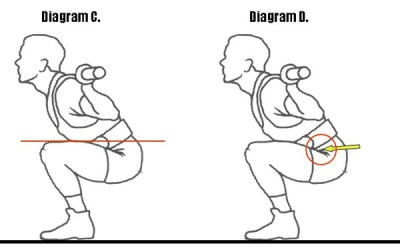
\includegraphics[scale=0.30]{squat-depth.jpg}\\
The hip crease must be below the top of the knee joint. 
\end{center}
\begin{center}
Figure 2: Bench Depth \\
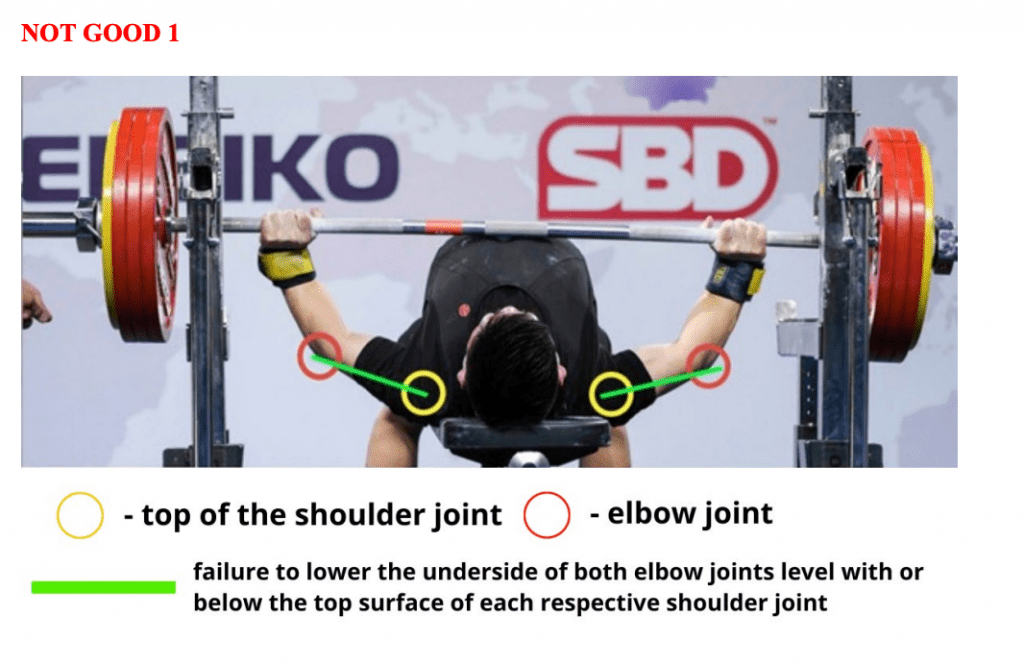
\includegraphics[scale=0.25]{bench-depth.png}\\
The elbow joint must be below the top of the shoulder joint.  
\end{center}
\section{Problem Statement}
How do we make powerlifting judging more objective, rather than subject to a human judge's perception?
\section{Motivation}
Sometimes, judging in Powerlifting can be subjective, because it is the perception of the judges that counts.  An innattentive or unfocused judge may not see if the lift was performed to the set standard, and may very well red-light a good lift, and vice-versa. It is possible that a seasoned judge may also make a bad call, and red-light a good lift, or white-light a bad lift. The motivation behind this project is to make judging lifts at a powerlifting meet more objective than subjective, which can be achieved with the use of computer vision technology. Instead of having judges, there are cameras with computers that perform the judging instead.  
\section{Proposed Solution}
\end{document}